\documentclass[11pt]{article}

\usepackage[margin=1in]{geometry}
\usepackage{fancyhdr}
\usepackage{amsmath,amsfonts,amsthm,bm}
\usepackage{amssymb}
\pagestyle{fancy}


\usepackage[T1]{fontenc}
\usepackage{CJKutf8}

\CJKencfamily{UTF8}{bkai} % 使用標楷體


\AtBeginDocument{%
    \begin{CJK}{UTF8}{bkai}} % 使用標楷體
    \AtEndDocument{%
    \clearpage\end{CJK}}
    
\usepackage{pgfplots} % for histogram plotting

\pgfplotsset{
  compat=newest,
  xlabel near ticks,
  ylabel near ticks
}
    
\usepackage{pgf,tikz}
\usepackage{mathrsfs}
\usetikzlibrary{arrows}
\usetikzlibrary[patterns]


\pgfdeclarepatternformonly[\GridSize]{MyGrid}{\pgfqpoint{-1pt}{-1pt}}{\pgfqpoint{4pt}{4pt}}{\pgfqpoint{\GridSize}{\GridSize}}%
{
  \pgfsetlinewidth{0.3pt}
  \pgfpathmoveto{\pgfqpoint{0pt}{0pt}}
  \pgfpathlineto{\pgfqpoint{0pt}{3.1pt}}
  \pgfpathmoveto{\pgfqpoint{0pt}{0pt}}
  \pgfpathlineto{\pgfqpoint{3.1pt}{0pt}}
  \pgfusepath{stroke}
}

\pgfdeclarepatternformonly[\GridSize]{MyGrid2}{\pgfqpoint{-1pt}{-1pt}}{\pgfqpoint{4pt}{4pt}}{\pgfqpoint{\GridSize}{\GridSize}}%
{
  \pgfsetlinewidth{0.3pt}
  \pgfpathmoveto{\pgfqpoint{0pt}{0pt}}
  \pgfpathlineto{\pgfqpoint{0pt}{-30pt}}
  \pgfpathmoveto{\pgfqpoint{0pt}{0pt}}
  \pgfpathlineto{\pgfqpoint{-30pt}{0pt}}
  \pgfusepath{stroke}
}

\newdimen\GridSize
\tikzset{
    GridSize/.code={\GridSize=#1},
    GridSize=3pt
}



\definecolor{qqqqff}{rgb}{0.,0.,1.}
\definecolor{ffqqqq}{rgb}{1.,0.,0.}
\definecolor{qqwuqq}{rgb}{0.,0.39215686274509803,0.}
\definecolor{cqcqcq}{rgb}{0.7529411764705882,0.7529411764705882,0.7529411764705882}

\usepackage{enumitem}
\usepackage{fancybox}
\usepackage{sectsty}
\allsectionsfont{\centering}
\PassOptionsToPackage{hyphens}{url}\usepackage[colorlinks=true, urlcolor=black, hyperfootnotes=false]{hyperref}

\lhead{Machine Learning Techniques (NTU, Spring 2017)}
\chead{}
\rhead{王冠鈞(b03902027)}



\begin{document}


\section*{Homework \#1}
\subsection*{Answer Sheet}
\begin{center}
DEADLINE: 04/11/2017, 14:00\\
INSTRUCTOR:  Hsuan-Tien Lin\\[0.5cm]
王冠鈞 b03902027
\end{center}


\begin{enumerate}[label=\textbf{\arabic*}.]
	\item The equation of the hyperplane is:\footnote{In this and the following 3 questions, I used the \texttt{cvxopt} package in python to compute the answers and I used Geogebra to visualize the results.}
	\[z_1 = 4\]
	To get this result, we have to first transform all $\mathbf{x_i}$ vectors with $\phi_1(\mathbf{x}), \phi_2(\mathbf{x})$, to the points in the $\mathcal{Z}$ space, say $\mathbf{z_i}$. Then apply the linear SVM optimization problem, and solve it with a QP solver, which can get:
	\[(b, \mathbf{w}) = (-4, (1, 0))\]
	Thus the equation of the hyperplane is show as above.\par 
	Also, we can plot all the transformed points $\mathbf{z_i}$ on the $\mathcal{Z}$ space, as shown below:
	
	
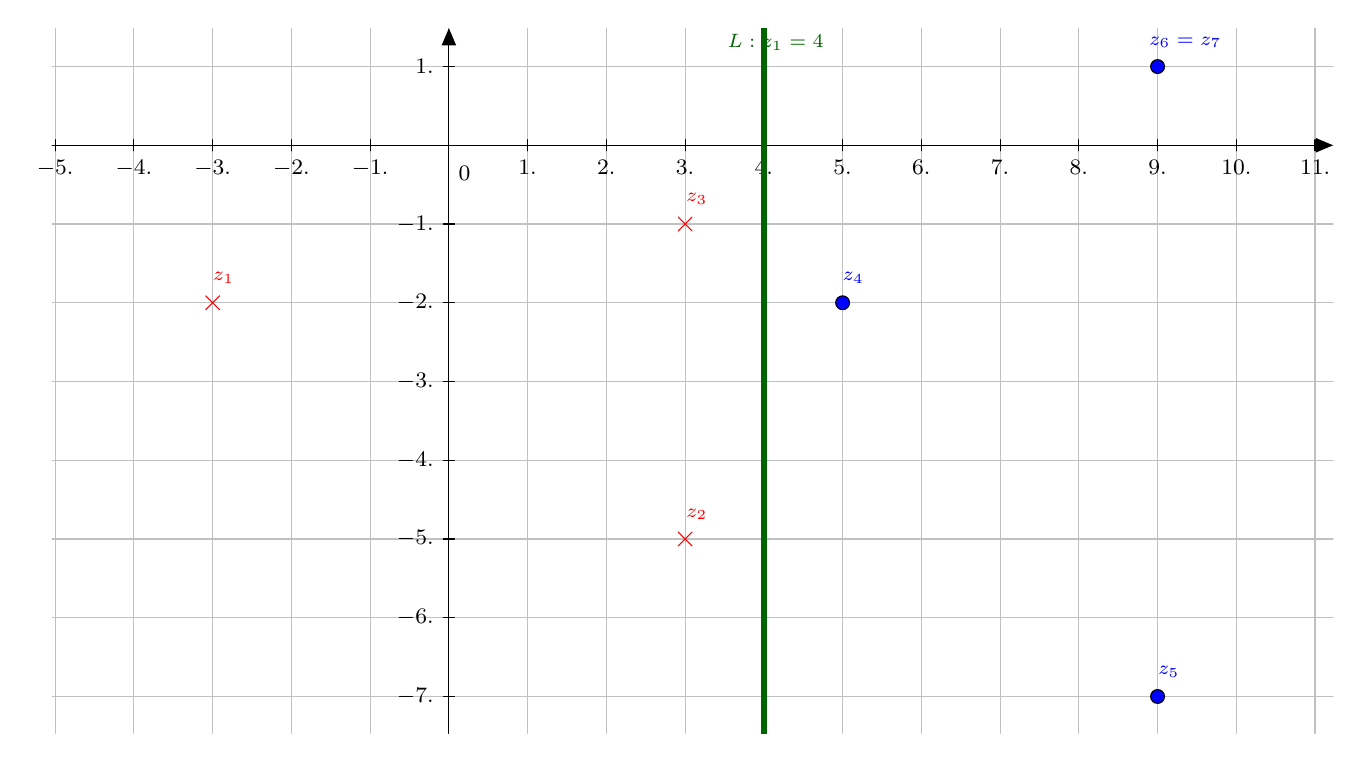
\begin{tikzpicture}[line cap=round,line join=round,>=triangle 45,x=1.0cm,y=1.0cm,scale=1]
\draw [color=cqcqcq,, xstep=1.0cm,ystep=1.0cm] (-5.03758440206431,-7.468540320924536) grid (11.22816455979174,1.4865916902443728);
\draw[->,color=black] (-5.03758440206431,0.) -- (11.22816455979174,0.);
\foreach \x in {-5.,-4.,-3.,-2.,-1.,1.,2.,3.,4.,5.,6.,7.,8.,9.,10.,11.}
\draw[shift={(\x,0)},color=black] (0pt,2pt) -- (0pt,-2pt) node[below] {\footnotesize $\x$};
\draw[->,color=black] (0.,-7.468540320924536) -- (0.,1.4865916902443728);
\foreach \y in {-7.,-6.,-5.,-4.,-3.,-2.,-1.,1.}
\draw[shift={(0,\y)},color=black] (2pt,0pt) -- (-2pt,0pt) node[left] {\footnotesize $\y$};
\draw[color=black] (0pt,-10pt) node[right] {\footnotesize $0$};
\clip(-5.03758440206431,-7.468540320924536) rectangle (11.22816455979174,1.4865916902443728);
\draw [line width=2.pt,color=qqwuqq] (4.,-7.468540320924536) -- (4.,1.4865916902443728);
\begin{scriptsize}
\draw[color=qqwuqq] (4.149274731263394,1.3071900472827251) node {$L: z_1 = 4$};
\draw [color=ffqqqq] (-3.,-2.)-- ++(-2.5pt,-2.5pt) -- ++(5.0pt,5.0pt) ++(-5.0pt,0) -- ++(5.0pt,-5.0pt);
\draw[color=ffqqqq] (-2.8623394811543323,-1.682837335411401) node {$z_1$};
\draw [color=ffqqqq] (3.,-5.)-- ++(-2.5pt,-2.5pt) -- ++(5.0pt,5.0pt) ++(-5.0pt,0) -- ++(5.0pt,-5.0pt);
\draw[color=ffqqqq] (3.1476155580608616,-4.687814855018997) node {$z_2$};
\draw [color=ffqqqq] (3.,-1.)-- ++(-2.5pt,-2.5pt) -- ++(5.0pt,5.0pt) ++(-5.0pt,0) -- ++(5.0pt,-5.0pt);
\draw[color=ffqqqq] (3.1476155580608616,-0.681178162208869) node {$z_3$};
\draw [fill=qqqqff] (5.,-2.) circle (2.5pt);
\draw[color=qqqqff] (5.135983767552456,-1.682837335411401) node {$z_4$};
\draw [fill=qqqqff] (9.,-7.) circle (2.5pt);
\draw[color=qqqqff] (9.142620460362586,-6.691133201424062) node {$z_5$};
\draw [fill=qqqqff] (9.,1.) circle (2.5pt);
\draw[color=qqqqff] (9.351922377151174,1.3071900472827251) node {$z_6 = z_7$};
\end{scriptsize}
\end{tikzpicture}
And via observation, we can easily find that the equation $z_1 = 4$ is most likely the hyperplane that separates the data, and only $\mathbf{z_2}, \mathbf{z_3}, \mathbf{z_4}$ determines the hyperplane.
	
	\item Instead of using the non-linear transform functions, we use a kernel function to do transformations in this question. Different from the previous question, we should use the first two steps of Kernel Hard-Margin SVM Algorithm to solve the optimal $\bm{\alpha}$. After feeding all necessary data to the QP solver, we can get the optimal $\bm{\alpha}$\footnote{The solutions from \texttt{cvxopt} are basically numerical values: \texttt{[2.081018335064783e-09, 0.4666666707571926, 0.4666666707571876, 0.5333333377102002, 0.20000000265577686, 0.2000000026557744, 5.736471702536082e-10]}, and I regard those with very low power as 0, and consider others to be rational numbers. }: \[\bm{\alpha} = (0, \frac{7}{15}, \frac{7}{15}, \frac{8}{15}, \frac{1}{5}, \frac{1}{5}, 0)\]
	And according to this result, the vectors $\mathbf{x_2}, \mathbf{x_3}, \mathbf{x_4}, \mathbf{x_5}, \mathbf{x_6}$ are support vectors.
	
	\item From the third step of the Kernel Hard-Margin SVM Algorithm we can get $b = -\frac{5}{3}$. And according to the last step\footnote{$g_{\mathrm{SVM}}(\mathbf{x})=\text{sign}\left( \Sigma_{\text{SV indices n}}\ \alpha_n y_n K(\mathbf{x_n}, \mathbf{x}) + b \right)$}, the non-linear curve should be: \[-\frac{7}{15}(2+x_2)^2-\frac{7}{15}(2-x_2)^2+\frac{8}{15}(2-x_1)^2+\frac{1}{5}(2+2x_2)^2+\frac{1}{5}(2-2x_2)^2-\frac{5}{3}=0\]
	\[ \Rightarrow\frac{1}{15}(8x_1^2-32x_1+10x_2^2-25)=0\]
	
	\item As the picture shown below (the dotted area denotes the points that $y = -1$), the (parabolic) curve $C_1$ is the non-linear curve from Question 1 (directly from $4 = \phi_1(\mathbf{x})=2x_2^2-4x_1+1$) and the (elliptic) curve  $C_2$ from Question 3. It's obvious that they are actually different ones since the transformation functions are basically different from each other.
	
	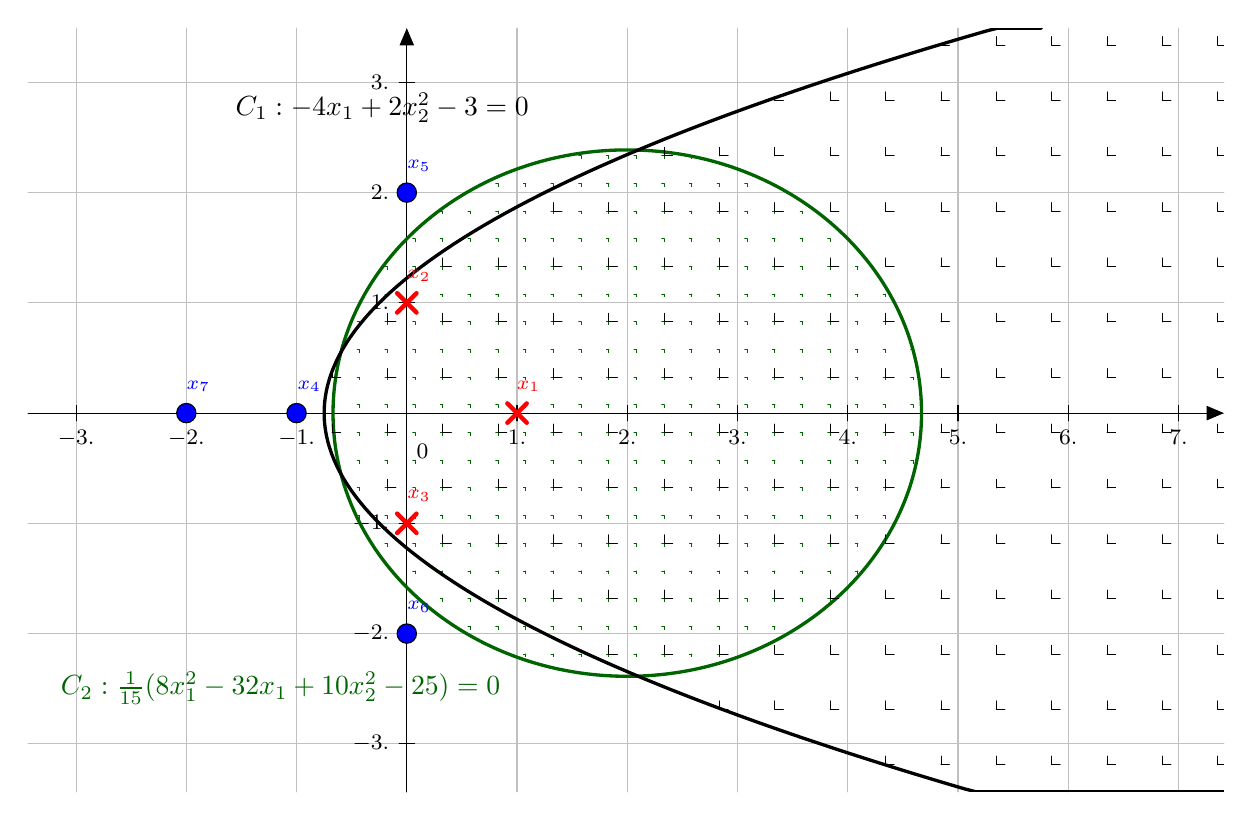
\begin{tikzpicture}[line cap=round,line join=round,>=triangle 45,x=1.0cm,y=1.0cm, scale=1.4, grid/.style={pattern=MyGrid}]
\draw [color=cqcqcq,, xstep=1.0cm,ystep=1.0cm] (-3.4342580691585094,-3.4351273859593627) grid (7.412238479424276,3.491366678647318);
\draw[->,color=black] (-3.4342580691585094,0.) -- (7.412238479424276,0.);
\foreach \x in {-3.,-2.,-1.,1.,2.,3.,4.,5.,6.,7.}
\draw[shift={(\x,0)},color=black] (0pt,2pt) -- (0pt,-2pt) node[below] {\footnotesize $\x$};
\draw[->,color=black] (0.,-3.4351273859593627) -- (0.,3.491366678647318);
\foreach \y in {-3.,-2.,-1.,1.,2.,3.}
\draw[shift={(0,\y)},color=black] (2pt,0pt) -- (-2pt,0pt) node[left] {\footnotesize $\y$};
\draw[color=black] (0pt,-10pt) node[right] {\footnotesize $0$};
\clip(-3.4342580691585094,-3.4351273859593627) rectangle (7.412238479424276,3.491366678647318);
%\draw [rotate around={0.:(2.,0.)},line width=1.2pt,color=qqwuqq,fill=qqwuqq,pattern=north west lines,pattern color=qqwuqq] (2.,0.) ellipse (2.669269563007828cm and 2.3874672772626644cm);
\draw [rotate around={0.:(2.,0.)},line width=1.2pt,color=qqwuqq,fill=qqwuqq,GridSize=10pt, pattern=MyGrid2,pattern color=qqwuqq] (2.,0.) ellipse (2.669269563007828cm and 2.3874672772626644cm);
\draw[line width=1.2pt,fill=black,GridSize=20pt, pattern=MyGrid,pattern color=black](5.7552281592896115,3.491366678647318)--(5.555087813648149,3.491366678647318)--(5.456190287161838,3.491366678647318)--(5.358074760157042,3.491366678647318)--(5.260741232633762,3.4672009184965162)--(5.164188998816293,3.439240908153813)--(5.068418764480338,3.411280897811109)--(4.973429823850194,3.3833208874684058)--(4.87922358847727,3.355360877125702)--(4.785797941034452,3.3274008667829986)--(4.693154998848853,3.299440856440295)--(4.601293350369065,3.2714808460975915)--(4.510213701370793,3.2435208357548877)--(4.4199160518540355,3.2155608254121844)--(4.330399696043089,3.1876008150694806)--(4.2416653397136574,3.159640804726777)--(4.153712277090036,3.1316807943840734)--(4.06654121394793,3.10372078404137)--(3.9801521502873394,3.0757607736986663)--(3.894545086108264,3.047800763355963)--(3.809719315634999,3.019840753013259)--(3.725674838867544,2.991880742670556)--(3.64241306735731,2.963920732327852)--(3.559932589552886,2.9359607219851487)--(3.4782341112299773,2.908000711642445)--(3.397316926612879,2.8800407012997415)--(3.317182447253001,2.8520806909570378)--(3.2378285558232283,2.8241206806143344)--(3.159257369650676,2.7961606702716306)--(3.0814674771839337,2.7682006599289273)--(3.0044595841987074,2.7402406495862235)--(2.9282329849192905,2.71228063924352)--(2.8527883851213893,2.6843206289008164)--(2.778125784805004,2.656360618558113)--(2.7042451839701336,2.628400608215409)--(2.6311458768410736,2.600440597872706)--(2.5588278634178234,2.572480587530002)--(2.4872925552517944,2.5445205771872987)--(2.416538540791575,2.516560566844595)--(2.346566525812871,2.4886005565018916)--(2.277375804539978,2.460640546159188)--(2.208967435636452,2.4326805358164845)--(2.141340360438737,2.4047205254737807)--(2.074495284722537,2.3767605151310773)--(2.0084318555999996,2.3488005047883735)--(1.943150425958978,2.32084049444567)--(1.8786502900237663,2.2928804841029664)--(1.8149325064579227,2.264920473760263)--(1.7519960165978894,2.2369604634175593)--(1.6898415262193713,2.209000453074856)--(1.628468682434516,2.181040442732152)--(1.5678778381311764,2.153080432389449)--(1.5080682875336466,2.125120422046745)--(1.4490407364176323,2.0971604117040417)--(1.3907951847831337,2.069200401361338)--(1.3333312797422976,2.0412403910186345)--(1.220748409441614,1.9853203703332274)--(1.1112928312912864,1.9294003496478203)--(1.004964192403463,1.8734803289624131)--(0.9017628456659956,1.817560308277006)--(0.8016880853031796,1.7616402875915989)--(0.7047409699785726,1.7057202669061917)--(0.6109204410286166,1.6498002462207846)--(0.5202272042290171,1.5938802255353774)--(0.43266090669192137,1.5379602048499703)--(0.3482215484173294,1.4820401841645632)--(0.2669094822930938,1.426120163479156)--(0.18872435543136193,1.370200142793749)--(0.11366616783213385,1.3142801221083418)--(0.04173491949540951,1.2583601014229346)--(-0.027069036690958413,1.2024400807375275)--(-0.09274570072696992,1.1465200600521204)--(-0.15529577838833034,1.0906000393667132)--(-0.21471856389933433,1.034680018681306)--(-0.27101441014783456,0.978759997995899)--(-0.3241833171338311,0.9228399773104918)--(-0.37422493196947115,0.8669199566250847)--(-0.4211396075426075,0.8109999359396776)--(-0.4649269909653874,0.7550799152542704)--(-0.5055877880135162,0.6991598945688633)--(-0.5431212929112886,0.6432398738834562)--(-0.577527682102631,0.587319853198049)--(-0.6088071320314695,0.5313998325126419)--(-0.6369594662538781,0.4754798118272347)--(-0.6619848612137827,0.41955979114182756)--(-0.6838831404672575,0.36363977045642043)--(-0.7026543040143021,0.30771974977101335)--(-0.7182985282988429,0.2517997290856062)--(-0.7308156368769536,0.19587970840019905)--(-0.7402056297486342,0.13995968771479192)--(-0.7464686833578111,0.0840396670293848)--(-0.7496046212605579,0.02811964634397766)--(-0.749613619900801,-0.027800374341429474)--(-0.7464955028346141,-0.0837203950268366)--(-0.740250270061997,-0.13964041571224373)--(-0.7308780980268761,-0.19556043639765086)--(-0.7183788102853251,-0.251480457083058)--(-0.7027524068373442,-0.30740047776846513)--(-0.6839990641268594,-0.36332049845387226)--(-0.6621186057099445,-0.4192405191392794)--(-0.6371112080305259,-0.47516053982468653)--(-0.6089766946446772,-0.5310805605100937)--(-0.5777152419963247,-0.5870005811955008)--(-0.5433264971976159,-0.6429206018809079)--(-0.5058108131364033,-0.6988406225663151)--(-0.4651680133687606,-0.7547606432517222)--(-0.4213982743386142,-0.8106806639371293)--(-0.374501596045964,-0.8666006846225365)--(-0.3244776256029574,-0.9225207053079436)--(-0.271326715897447,-0.9784407259933507)--(-0.21504886692943292,-1.0343607466787579)--(-0.15564407869891506,-1.090280767364165)--(-0.09311199831804078,-1.1462007880495722)--(-0.027452625786810077,-1.2021208087349793)--(0.041333333119071704,-1.2580408294203864)--(0.1132465841753099,-1.3139608501057936)--(0.18828677449405185,-1.3698808707912007)--(0.2664542569631502,-1.4258008914766078)--(0.3477483258068997,-1.481720912162015)--(0.43216968680100554,-1.537640932847422)--(0.5197183399454678,-1.5935609535328292)--(0.6103935794645812,-1.6494809742182364)--(0.704196111134051,-1.7054009949036435)--(0.8011259349538772,-1.7613210155890506)--(0.9011823451483545,-1.8172410362744578)--(1.0043660474931881,-1.873161056959865)--(1.1106770419883782,-1.929081077645272)--(1.2201146228582196,-1.9850010983306792)--(1.3326794958784172,-2.0409211190160863)--(1.3901345787229364,-2.0688811293587897)--(1.4483713081611185,-2.0968411397014934)--(1.507390037080816,-2.124801150044197)--(1.5671904125941762,-2.1527611603869006)--(1.6277724347011995,-2.180721170729604)--(1.6891361034018852,-2.2086811810723077)--(1.7512817715840865,-2.236641191415011)--(1.8142094392478032,-2.264601201757715)--(1.87791840061733,-2.292561212100418)--(1.9424093614683722,-2.320521222443122)--(2.007681968913077,-2.3484812327858253)--(2.073736575839298,-2.376441243128529)--(2.140572829359181,-2.4044012534712325)--(2.2081907294727268,-2.4323612638139362)--(2.2765902761799355,-2.4603212741566396)--(2.34577182236866,-2.4882812844993434)--(2.415735015151047,-2.5162412948420467)--(2.486480207414949,-2.5442013051847505)--(2.5580070462725146,-2.572161315527454)--(2.6303151788358896,-2.6001213258701577)--(2.7034060166564857,-2.628081336212861)--(2.777278148182892,-2.656041346555565)--(2.8519315734151083,-2.684001356898268)--(2.9273669981288397,-2.711961367240972)--(3.003584422324087,-2.7399213775836753)--(3.0805838460008497,-2.767881387926379)--(3.1583645633834223,-2.7958413982690824)--(3.2369272802475106,-2.823801408611786)--(3.316271290817409,-2.8517614189544895)--(3.3963980066445276,-2.8797214292971933)--(3.4773060161774567,-2.9076814396398967)--(3.558995319416196,-2.9356414499826005)--(3.6414666221364507,-2.963601460325304)--(3.7247199243382205,-2.9915614706680076)--(3.808755226021506,-3.019521481010711)--(3.893571821410602,-3.0474814913534147)--(3.979170416281213,-3.075441501696118)--(4.065550304857634,-3.103401512038822)--(4.152712192915571,-3.131361522381525)--(4.240656080455023,-3.159321532724229)--(4.329381967475991,-3.1872815430669323)--(4.4188891482027675,-3.215241553409636)--(4.5091783284110605,-3.2432015637523395)--(4.600248802325164,-3.2711615740950433)--(4.692101275720782,-3.2991215844377466)--(4.7847357485979165,-3.3270815947804504)--(4.878152220956566,-3.3550416051231537)--(4.972349987021025,-3.3830016154658575)--(5.067329752567001,-3.410961625808561)--(5.163090811818785,-3.4351273859593627)--(5.259633870552086,-3.4351273859593627)--(5.356958928766902,-3.4351273859593627)--(5.553954337865375,-3.4351273859593627)--(7.527872770986992,-3.4351273859593627)--(7.527872770986992,3.491366678647318);
\draw (-1.6419265499364073,2.9941392249276397) node[anchor=north west] {$C_1: -4x_1+2x_2^2-3=0$};
\draw [color=qqwuqq](-3.2261163443456202,-2.255657612019661) node[anchor=north west] {$C_2: \frac{1}{15}(8x_1^2-32x_1+10x_2^2-25)=0$};
\begin{scriptsize}
\draw [ultra thick,color=ffqqqq] (1.,0.)-- ++(-2.5pt,-2.5pt) -- ++(5.0pt,5.0pt) ++(-5.0pt,0) -- ++(5.0pt,-5.0pt);
\draw[ultra thick,color=ffqqqq] (1.1043878746781037,0.24204308573500205) node {$x_1$};
\draw [ultra thick,color=ffqqqq] (0.,1.)-- ++(-2.5pt,-2.5pt) -- ++(5.0pt,5.0pt) ++(-5.0pt,0) -- ++(5.0pt,-5.0pt);
\draw[color=ffqqqq] (0.10993296723874402,1.24806142233063) node {$x_2$};
\draw [ultra thick,color=ffqqqq] (0.,-1.)-- ++(-2.5pt,-2.5pt) -- ++(5.0pt,5.0pt) ++(-5.0pt,0) -- ++(5.0pt,-5.0pt);
\draw[color=ffqqqq] (0.10993296723874402,-0.7524118217043545) node {$x_3$};
\draw [fill=qqqqff] (-1.,0.) circle (2.5pt);
\draw[color=qqqqff] (-0.8845219402006158,0.24204308573500205) node {$x_4$};
\draw [fill=qqqqff] (0.,2.) circle (2.5pt);
\draw[color=qqqqff] (0.10993296723874402,2.2425163297699866) node {$x_5$};
\draw [fill=qqqqff] (0.,-2.) circle (2.5pt);
\draw[color=qqqqff] (0.10993296723874402,-1.7584301582999828) node {$x_6$};
\draw [fill=qqqqff] (-2.,0.) circle (2.5pt);
\draw[color=qqqqff] (-1.8905402767962474,0.24204308573500205) node {$x_7$};
\end{scriptsize}
\end{tikzpicture}


	\item Consider for all data $\mathbf{x_i}$, if they are correctly separated, we will set $\xi_i' < 0$, which means the ``correctness'' of a point (if a point is correctly separated and is further from the separation line, the value will be much more negative), then we can get:
	\[\frac{1}{2}\mathbf{w}^T\mathbf{w}+C\sum_{n=1}^N\xi_n'^2 > \frac{1}{2}\mathbf{w}^T\mathbf{w}+C\sum_{n=1}^N\xi_n^2, \forall\xi_i \geq 0\]
	That is, to minimize the objective function, those ``correct'' data should set their $\xi$s to $0$ instead of negative. Thus, the constraint ``$\xi_n \geq 0, \text{for } n = 1, 2, \cdots,N$'' is unnecessary here.\par 
	We can also compare with the linear-penalty model ($P_1$). If we allow some $\xi_i < 0$, then the penalty may be eliminated by the correct data, which may lower the incentive to make less mistakes. However in the current model ($P_2'$), negative $\xi_i$s will merely make the objective function further from optimum, so without such constraint, the optimum will still not make any $\xi_i$ become negative.
	
	\item As the steps demonstrated in the Dual SVM lecture, we can easily write down the Lagrange function:
	\[\mathcal{L}((b, \mathbf{w}, \bm{\xi}), \bm{\alpha}) = \frac{1}{2}\mathbf{w}^T\mathbf{w}+C\sum_{n=1}^N \xi_n^2 + \sum_{n=1}^N\alpha_n (1-\xi_n - y_n (\mathbf{w}^T\mathbf{x}_n+b))\]
	
	\item The three-step simplification, which eliminates $b, \bm{\xi}, \mathbf{w}$, is shown below:
	\begin{enumerate}
		\item $\frac{\partial\mathcal{L}((b, \mathbf{w}, \bm{\xi}), \bm{\alpha})}{\partial b} = 0 = -\sum_{n=1}^N\alpha_n y_n$, then we can eliminate $b$ by adding the constraint $\sum_{n=1}^N\alpha_n y_n = 0$:
		\[\underset{\alpha_n \geq 0,\ \sum y_n \alpha_n = 0}\max \left( \underset{\mathsf{\mathbf{w}, \bm{\xi}}}\min \frac{1}{2}\mathbf{w}^T\mathbf{w}+C\sum_{n=1}^N \xi_n^2 + \sum_{n=1}^N\alpha_n (1-\xi_n - y_n (\mathbf{w}^T\mathbf{x}_n)) \right)\]
		
		\item $\frac{\partial\mathcal{L}((b, \mathbf{w}, \bm{\xi}), \bm{\alpha})}{\partial \xi_n} = 0 = 2C\xi_n - \alpha_n \Rightarrow \xi_n = \frac{\alpha_n}{2C}$, then we can eliminate $\bm{\xi}$ with $\bm{\alpha}$ by replacing $\xi_n$ with $\frac{\alpha_n}{2C}$:
		\[\underset{\alpha_n \geq 0,\ \sum y_n \alpha_n = 0}\max \left( \underset{\mathsf{\mathbf{w}}}\min \frac{1}{2}\mathbf{w}^T\mathbf{w}+\sum_{n=1}^N \frac{\alpha_n^2}{4C} + \sum_{n=1}^N\alpha_n (1- \frac{\alpha_n}{2C} - y_n (\mathbf{w}^T\mathbf{x}_n)) \right)\]
		
		\item $\frac{\partial\mathcal{L}((b, \mathbf{w}, \bm{\xi}), \bm{\alpha})}{\partial w_i} = 0 = w_i - \sum_{n=1}^N \alpha_n y_n x_{n, i}$, then we can eliminate $\mathbf{w}$ with constraint $\mathbf{w}=\sum_{n=1}{N}\alpha_n y_n \mathbf{x}_n$:
		\[\underset{\alpha_n \geq 0,\ \sum y_n \alpha_n = 0, \mathbf{w} = \sum \alpha_n y_n \mathbf{x}_n}\max \left( \underset{\mathsf{\mathbf{w}}}\min \frac{1}{2}\mathbf{w}^T\mathbf{w}+\sum_{n=1}^N \frac{\alpha_n^2}{4C} + \sum_{n=1}^N\alpha_n (1- \frac{\alpha_n}{2C}) - \mathbf{w}^T\mathbf{w} \right)\]
		\[\Longleftrightarrow \underset{\alpha_n \geq 0,\ \sum y_n \alpha_n = 0, \mathbf{w} = \sum \alpha_n y_n \mathbf{x}_n}\max -\frac{1}{2} \| \sum_{n=1}^N \alpha_n y_n \mathbf{x}_n \|^2 - \sum_{n=1}^N \frac{\alpha_n^2}{4C} + \sum_{n=1}^N \alpha_n \]
		\item And finally, 
		\[\underset{\alpha}\min\ \frac{1}{2} \sum_{n=1}^N \sum_{m=1}^N \alpha_n \alpha_m y_n y_m \mathbf{x}_n^T \mathbf{x}_m + \frac{1}{4C}\sum_{n=1}^N \alpha_n^2 - \sum_{n=1}^N \alpha_n\]
		, which is the dual problem we are seeking.
	\end{enumerate}
	
	\item When using $\mathbf{z}_n = \phi(\mathbf{x}_n)$, we will be able to transform the current space to $\mathcal{Z}$ space non-linearly, and it will make the separating curve in $\mathcal{X}$ space become a non-linear curve. \par 
	The optimization problem when using a kernel $K(\mathbf{x}_n, \mathbf{x}_m)$ is similar to the problem above, with only a few variables replaced:
	\[\underset{\alpha}\min\ \frac{1}{2} \sum_{n=1}^N \sum_{m=1}^N \alpha_n \alpha_m y_n y_m K(\mathbf{x}_n, \mathbf{x}_m) + \frac{1}{4C}\sum_{n=1}^N \alpha_n^2 - \sum_{n=1}^N \alpha_n\]
	
	\item 
	\begin{enumerate}[label={[\textbf{\alph*}]}]
		\item \textit{Not necessarily valid.} I've found a counterexample by using Wolfram Alpha. First, the matrix $\left(\begin{array}{cc} 0.2 & 0.3 \\ 0.3 & 0.5\end{array}\right)$ is symmetric, positive semidefinite, and is from some kernel $K_1$ with $0 < K_1 < 1$. However, the matrix $\left(\begin{array}{cc} 1 - 0.2 & 1 - 0.3 \\ 1 - 0.3 & 1 - 0.5\end{array}\right) = \left(\begin{array}{cc} 0.8 & 0.7 \\ 0.7 & 0.5\end{array}\right)$ is not positive semidefinite. Thus the new kernel $K'(\mathbf{x}, \mathbf{x'})$ is not necessarily valid.
		
		\item \textit{Valid.} Since $0 < 1 - K_1(\mathbf{x}, \mathbf{x'}) < 1$, its zero-th power will always become $1$. Thus the $M_K$ will be a matrix where all terms $= 1$, and it's apparently symmetric. As for positive semi-definiteness, consider the operation $\mathbf{z}^TM_K\mathbf{z} = \sum\sum z_i z_j m_{ij} = \sum\sum z_i z_j = (\sum z_i)^2 \geq 0$. Thus it is positive semi-definiteness and $K$ is also valid.
		
		\item I guess that it is valid, but I have no idea how to prove it.
		
		\item According to the operations of kernels, [\textbf{d}] can be regarded as the power of 2 of the kernel in [\textbf{c}], and the multiplicaton of two valid kernels is also valid; that is, if [\textbf{c}] is valid, so is [\textbf{d}].
	\end{enumerate}
	
	\item \begin{proof}
	Consider the original problem of Soft-Margin SVM Dual:
	\[\begin{array}{rl} (P)\ \underset{\bm{\alpha}}\min & \frac{1}{2} \sum_{n=1}^N \sum_{m=1}^N \alpha_n \alpha_m y_n y_m K(\mathbf{x}_n, \mathbf{x}_m) - \sum_{n=1}^N \alpha_n \\
	\text{subject to} & \sum_{n=1}^N y_n \alpha_n = 0; \\
	& 0 \leq \alpha_n \leq C, \text{for } n=1, 2, \cdots , N
	\end{array}\]
	Let the solution of $P$ be $\bm{\alpha^*}$ and the classifier $g_{\mathrm{SVM}}$ of this SVM is:
	\[g_{\mathrm{SVM}}(\mathbf{x}) = \text{sign}\left( \sum_{\mathsf{SV}}\alpha_n y_n K(\mathbf{x}_n, \mathbf{x}) + b \right)\]
	\[ = \text{sign}\left( \sum_{\mathsf{SV}}\alpha_n y_n K(\mathbf{x}_n, \mathbf{x}) +y_s - \sum_{\mathsf{SV}}\alpha_n y_n K(\mathbf{x}_n, \mathbf{x}_s) \right)\]
	Now, when we use the new kernel $\tilde{K}(\mathbf{x}, \mathbf{x'}) = pK(\mathbf{x}, \mathbf{x'})+q, p>0, q\geq 0$, the new classifier $g_{\mathrm{SVM}}'$ will be (let $\bm{\alpha'}$ be the new solution):
	\[g_{\mathrm{SVM}}' = \text{sign}\left( \sum_{\mathsf{SV}}\alpha_n' y_n \tilde{K}(\mathbf{x}_n, \mathbf{x}) +y_s - \sum_{\mathsf{SV}}\alpha_n' y_n \tilde{K}(\mathbf{x}_n, \mathbf{x}_s) \right)\]
	\[ = \text{sign}\left( \sum_{\mathsf{SV}}\alpha_n' y_n pK(\mathbf{x}_n, \mathbf{x}) +y_s - \sum_{\mathsf{SV}}\alpha_n' y_n pK(\mathbf{x}_n, \mathbf{x}_s) \right)\]
	\[ = \text{sign}\left( \sum_{\mathsf{SV}}(p\alpha_n') y_n K(\mathbf{x}_n, \mathbf{x}) +y_s - \sum_{\mathsf{SV}}(p\alpha_n') y_n K(\mathbf{x}_n, \mathbf{x}_s) \right)\]
	That is, if $g_{\mathrm{SVM}}' = g_{\mathrm{SVM}}$, then $p\alpha_n' = \alpha_n^*, (\text{for every } n)$ could be the solution: the new solutions  $\bm{\alpha'}$ are shrunken by $p$ times from $\bm{\alpha}$. Geometrically, we can regard the hyperplanes of new objective functions and constraints as being shrunken by $p$ times, so that the new solutions set will be $\bm{\alpha'}$ (which is also shrunken by $p$ times):
	\[\begin{array}{rl} (P')\ \underset{\bm{\alpha}}\min & \frac{1}{2} \sum_{n=1}^N \sum_{m=1}^N \alpha_n' \alpha_m' y_n y_m (pK(\mathbf{x}_n, \mathbf{x}_m)+q) - \sum_{n=1}^N \alpha_n'  \\
	\text{subject to} & \frac{1}{p}\sum_{n=1}^N y_n \alpha_n' = 0; \\
	& 0 \leq \alpha_n' \leq \frac{C}{p} = \tilde{C}, \text{for } n=1, 2, \cdots , N\\
	\text{where} & \alpha_i' = \frac{\alpha_i}{p}
	\end{array}\]
	Note that the objective now contains a new term $\frac{q}{2}\sum_{n=1}^N \sum_{m=1}^N\alpha_n' \alpha_m' y_n y_m$, but according to the constraint $\sum_{n=1}^N y_n \alpha_n' = 0$, the new term should always be 0. Thus all functions and constraints are in fact merely shrunken by $p$ times, and thus $\bm{\alpha'} = \frac{\bm{\alpha^*}}{p}$. In this situation $C$ is also shrunken by $p$ times, and thus we get $\tilde{C} = \frac{C}{p}$.
%	Thus we get $p\alpha_n' = \alpha_n$ when $g_{\mathrm{SVM}}' = g_{\mathrm{SVM}}$.\par 
%	For those bounded support vectors $\mathbf{x}_s$, $\alpha_s = C = p\alpha_s' = p\tilde{C} \Rightarrow \tilde{C} = \frac{C}{p}$ 
	\end{proof}
	
	\item Histogram:\\
	\begin{tikzpicture}[font=\tiny]
    \begin{axis}[
      ybar,
      bar width=20pt,
      x=42pt,
      xlabel={$\log_{10} C$},
      ylabel={$\|\mathbf{w}\|$},
      ymin=0,
      ytick=\empty,
      xtick=data,
      axis x line=bottom,
      axis y line=left,
      enlarge x limits=0.2,
      symbolic x coords={-5, -3, -1, 1, 3},
      xticklabel style={anchor=base,yshift=-\baselineskip},
      nodes near coords={\pgfmathprintnumber\pgfplotspointmeta}
    ]
      \addplot[fill=white] coordinates {
        (-5, 0.001109) 
        (-3, 0.057525) 
        (-1, 5.473332) 
        (1, 12.985649)
        (3, 13.117025)
      };
      \end{axis}
  \end{tikzpicture}\\
  	From the graph above, it's easy to find that the $\|\mathbf{w}\|$ value increases as $\log_{10}C$ increases. The possible reason is that, according to the implicit constraint $\mathbf{w} = \sum_{n=1}^N \alpha_n y_n \mathbf{z}_n$, when $C$ increases, $\alpha_n$ may increase, and this will cause the absolute values some terms of $\mathbf{w}$ to be larger, which will make $\|\mathbf{w}\|$ larger. Some other findings are that the larger C is, the longer it computes\footnote{The \texttt{libsvm} package gives a warning at $C=1000$, stating that it has reached the maximum number of iterations.}, and that $\|\mathbf{w}\|$ grows fast at $\log_{10}C = -1$, but slowly at other points.

	\item Histogram:\\
	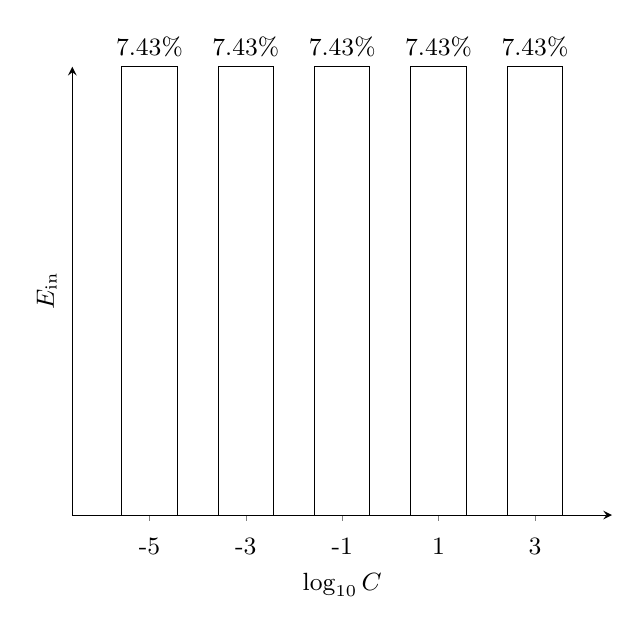
\begin{tikzpicture}[font=\small]
    \begin{axis}[
      ybar,
      bar width=20pt,
      xlabel={$\log_{10} C$},
      ylabel={$E_{\text{in}}$},
      ymin=0,
      ytick=\empty,
      xtick=data,
      axis x line=bottom,
      axis y line=left,
      enlarge x limits=0.2,
      symbolic x coords={-5, -3, -1, 1, 3},
      xticklabel style={anchor=base,yshift=-\baselineskip},
      nodes near coords={\pgfmathprintnumber\pgfplotspointmeta\%}
    ]
      \addplot[fill=white] coordinates {
        (-5, 7.433823) 
        (-3, 7.433823) 
        (-1, 7.433823) 
        (1, 7.433823)
        (3, 7.433823)
      };
      \end{axis}
  \end{tikzpicture}\\
  	What's interesting is that $E_{\text{in}}$ remains the same no matter what $C$ is. Perhaps it's because it has reached its maximum accuracy since $C$ is $10^{-5}$, and any more penalty on violations will not enable the model to make any less errors.

	\item Histogram:\\
	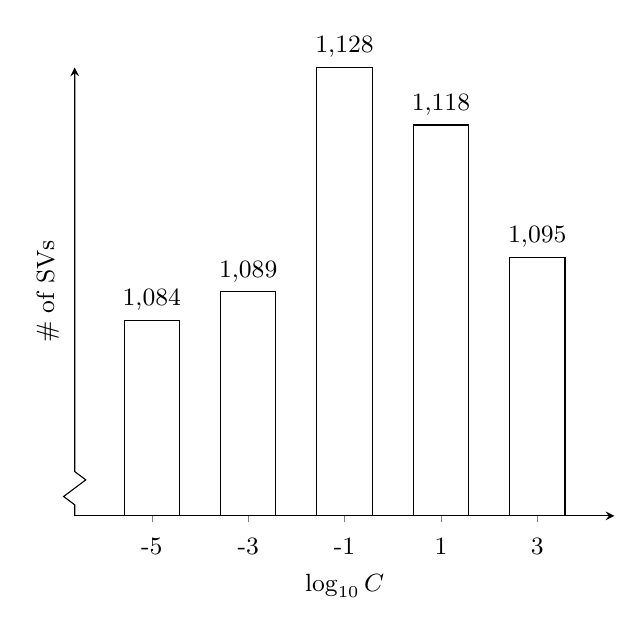
\begin{tikzpicture}[font=\small]
    \begin{axis}[
      ybar,
      bar width=20pt,
      xlabel={$\log_{10} C$},
      ylabel={\# of SVs},
      axis y discontinuity=crunch,
      ymin=1050,
      ytick=\empty,
      xtick=data,
      axis x line=bottom,
      axis y line=left,
      enlarge x limits=0.2,
      symbolic x coords={-5, -3, -1, 1, 3},
      xticklabel style={anchor=base,yshift=-\baselineskip},
      nodes near coords={\pgfmathprintnumber\pgfplotspointmeta}
    ]
      \addplot[fill=white] coordinates {
        (-5, 1084) 
        (-3, 1089) 
        (-1, 1128) 
        (1, 1118)
        (3, 1095)
      };
      \end{axis}
  \end{tikzpicture}\\
  	The result is that it reaches a peak when $C = 0.1$.

	\item Histogram:\\
	\begin{tikzpicture}[font=\tiny]
    \begin{axis}[
      ybar,
      bar width=20pt,
      xlabel={$\log_{10} C$},
      ylabel={distance},
      ymin=0,
      ytick=\empty,
      xtick=data,
      axis x line=bottom,
      axis y line=left,
      enlarge x limits=0.2,
      symbolic x coords={-3, -2, -1, 0, 1},
      xticklabel style={anchor=base,yshift=-\baselineskip},
      nodes near coords={\pgfmathprintnumber\pgfplotspointmeta}
    ]
      \addplot[fill=white] coordinates {
        (-3, 7.678389) 
        (-2, 0.768642) 
        (-1, 0.135644) 
        (0, 0.089335)
        (1, 0.043855)
      };
      \end{axis}
  \end{tikzpicture}\\
  	The distince decreases as the $\log_{10} C$ grows. According to the distance formula: $d(\mathbf{z}) = \frac{1}{\|\mathbf{w}\|} |\mathbf{w}^T\mathbf{z}+b|$, and consider a free support vector $\mathbf{x}_s$,  $|{w}^T\mathbf{z}+b| = |\sum_{\mathsf{SV}}\alpha_n y_n K(\mathbf{x}_n, \mathbf{x}_s) +y_s - \sum_{\mathsf{SV}}\alpha_n y_n K(\mathbf{x}_n, \mathbf{x}_s)| = |y_s| = 1$ Thus for any $\mathbf{x}_s$, the distance to the hyperplane will be $\frac{1}{\|\mathbf{w}\|}$ (reverse of $\|\mathbf{w}\|$), and I've mentioned that $\|\mathbf{w}\|$ may increase as $C$ increases, so it may also be the reason that the distance decreases as $C$ increases.

	\item Histogram:\\
	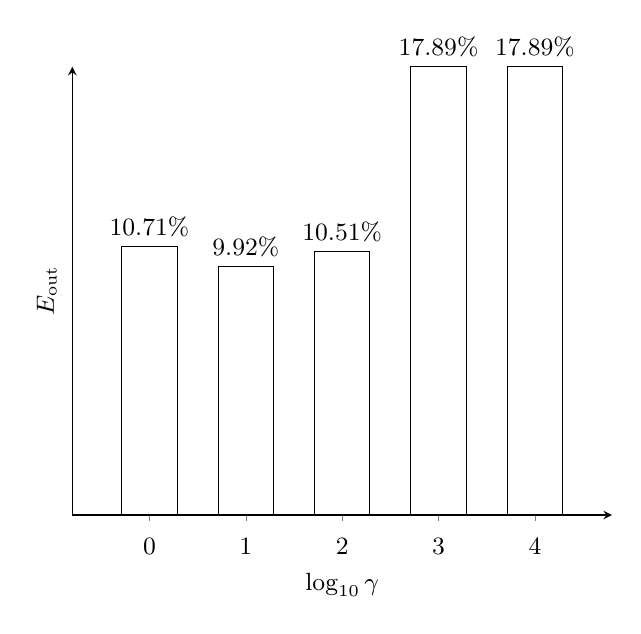
\begin{tikzpicture}[font=\small]
    \begin{axis}[
      ybar,
      bar width=20pt,
      xlabel={$\log_{10} \gamma$},
      ylabel={$E_{\text{out}}$},
      ymin=0,
      ytick=\empty,
      xtick=data,
      axis x line=bottom,
      axis y line=left,
      enlarge x limits=0.2,
      symbolic x coords={0,1,2,3, 4},
      xticklabel style={anchor=base,yshift=-\baselineskip},
      nodes near coords={\pgfmathprintnumber\pgfplotspointmeta\%}
    ]
      \addplot[fill=white] coordinates {
        (0, 10.712506) 
        (1, 9.915296) 
        (2, 10.513204) 
        (3, 17.887394)
        (4, 17.887394)
      };
    \end{axis}
  \end{tikzpicture}\\
  	According to the result, $E_{\text{out}}$ is generally higher when $\log_{10} \gamma$ is large, which means that out-sample errors are higher when we choose a large $\gamma$. A possible reason to this result is that large $\gamma$ values in a Guassian kernel may lead to overfitting, which is not good for data prediction, and thus cause high $E_{\text{out}}$.

	\item Histogram:\\
	\begin{tikzpicture}[font=\small]
    \begin{axis}[
      ybar,
      bar width=20pt,
      xlabel={$\log_{10} \gamma$},
      ylabel={chosen times},
      ymin=0,
      ytick=\empty,
      xtick=data,
      axis x line=bottom,
      axis y line=left,
      enlarge x limits=0.2,
      symbolic x coords={-1,0,1,2,3},
      xticklabel style={anchor=base,yshift=-\baselineskip},
      nodes near coords={\pgfmathprintnumber\pgfplotspointmeta}
    ]
      \addplot[fill=white] coordinates {
        (-1,0)
        (0,7)
        (1,67)
        (2,26)
        (3,0)
      };
    \end{axis}
  \end{tikzpicture}
	
	


\end{enumerate}

\end{document}